\section{Exercise 2: Ionospheric delay analysis}

Questions:
\begin{enumerate}
\item Justify the expressions used to depict the Ionospheric delay (see slides #16 to #18).
\item Justify the factors of 5.09 and 3.09 used in the P2-L2 and P1-L1 combinations to give the results of L1-L2 delay in metres.
\item Why is the STEC larger at low elevations?
\end{enumerate}


\textcolor{Red}{NOT WORKING}
\begin{figure}[H]
        \centering
        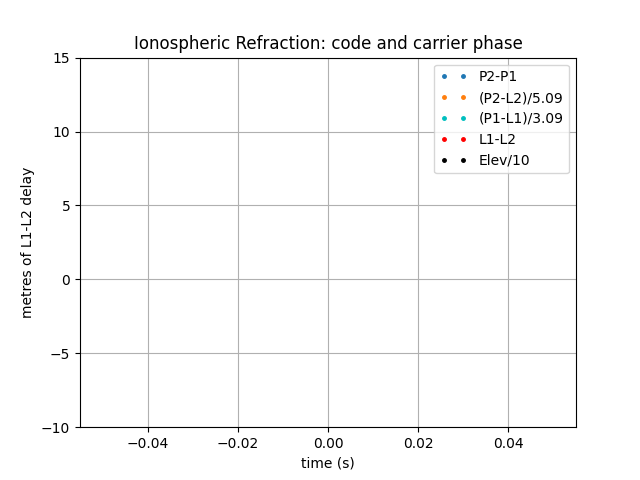
\includegraphics[scale=0.52]{sources/Figures/FIG_2/TUT2_Ex2a.png}
        \caption{}
        \label{fig:}
\end{figure}
